\documentclass[10pt]{article}
\usepackage[letterpaper,margin=0.70in]{geometry}
\usepackage[T1]{fontenc}
\usepackage{lmodern}
\usepackage{microtype}
\usepackage{booktabs}
\usepackage{graphicx}
\usepackage[dvipsnames]{xcolor}
\usepackage{hyperref}

\definecolor{NvidiaGreen}{HTML}{5C8F00}
\hypersetup{colorlinks=true,linkcolor=NvidiaGreen,urlcolor=NvidiaGreen,citecolor=NvidiaGreen}
\setlength{\parindent}{0pt}
\setlength{\parskip}{0.38em}
\setlength{\tabcolsep}{4.2pt}
\renewcommand{\arraystretch}{1.08}
\newcommand{\best}[1]{\textbf{\color{NvidiaGreen}#1}}

\title{\textbf{Topology-Aware Distributed Layerwise Offloading\\
for MiniMax-H3 on Eight NVIDIA B300 GPUs}}
\author{Shunyang Li\\\small Empirical Systems Research Note}
\date{9 August 2026}

\begin{document}
\maketitle

\begin{abstract}
We study how data parallelism (DP), sequence parallelism (SP), and distributed
layerwise offloading (DLO) interact for MiniMax-H3 video--audio generation on
one eight-GPU NVIDIA B300 node.  Three production-relevant routes are evaluated
with 20 measured 50-step text-to-video-and-audio (T2VA) waves across two engine
lifecycles.  DP1$\times$SP8 with AllGather minimizes wave latency
(P50/P95: 34.55/35.25 s), DP4$\times$SP2 with AllGather is the balanced point
(151.89 videos/h at P95 95.31 s), and DP8$\times$SP1 with rank-local DLO
maximizes throughput and minimizes energy (183.78 videos/h, 43.97 Wh/video).
The central result is that DLO mode is topology-dependent: AllGather improves
DP1 throughput by 129.4\%, offers only 2.2\% at DP4, and reduces DP8
throughput by 4.1\% while increasing the observed per-GPU memory peak from
20.03 to 94.03 GiB.  FL2VA and Ref2VA preserve the same
latency--throughput ordering.  These measurements reject a single global DLO
policy and motivate topology-aware deployment.
\end{abstract}

\textbf{Keywords:} diffusion inference; distributed layerwise offload; data
parallelism; sequence parallelism; video generation; B300; vLLM-Omni

\section{Introduction}

On a fixed multi-GPU node, sequence parallelism reduces one request's latency,
whereas data parallelism increases concurrent request capacity.  Distributed
layerwise offloading adds a second design axis: DP replicas may advance weights
through compatible collective waves (AllGather) or maintain rank-local weight
state and execute independent requests.  Communication, host-to-device
transfer, activation memory, and concurrency therefore change together.

This note asks three questions:
\textbf{RQ1}: Which DP$\times$SP configurations lie on the
latency--throughput frontier?
\textbf{RQ2}: At which topology does AllGather outperform rank-local DLO?
\textbf{RQ3}: Does the frontier persist under image- and audio-conditioned
generation?
vLLM-Omni supports diffusion and heterogeneous multimodal outputs
\cite{vllmomni}; recent changes harden collective DP waves \cite{pr5864} and
enable independent rank-local DP requests \cite{pr5911}.

\paragraph{Contributions.}
We provide (i) a full-step, two-lifecycle T2VA frontier with latency,
throughput, energy, and memory; (ii) a paired AllGather/rank-local comparison;
and (iii) FL2VA/Ref2VA transfer measurements with preserved wave-level data.

\section{Method}

\begin{table}[ht]
\centering
\caption{Controlled experimental configuration.}
\label{tab:setup}
\small
\begin{tabular}{@{}ll@{}}
\toprule
Dimension & Setting \\
\midrule
Node & 8$\times$ NVIDIA B300 SXM6 AC; NV18 full mesh; one NUMA domain \\
Model & MiniMax-H3 FL2VA / Ref2VA; BF16; \texttt{CUDNN\_ATTN} \\
Output & 768$\times$1344; 124 frames; stereo audio \texttt{[1,2,165600]} \\
DLO & \texttt{resident\_layers=0}; AllGather or rank-local; eager execution \\
Sampling & 50 requested steps (49 scheduler denoising updates) \\
T2VA & 1 full warmup/lifecycle; 5+15 measured waves; 2 lifecycles \\
FL2VA / Ref2VA & 1 full warmup; 5 measured waves per selected route \\
Telemetry & External \texttt{nvidia-smi}; 0.758 s median interval \\
\bottomrule
\end{tabular}
\end{table}

DP1, DP4, and DP8 generate one, four, and eight outputs per wave.  Throughput
is measured outputs divided by measured wave time.  Per-video energy is the
trapezoidal integral of summed eight-GPU board power divided by output count;
no idle baseline is subtracted.  We report empirical P50/P95 and CV.
The $n=20$ mean-latency t-intervals are descriptive because samples are
clustered within two engine lifecycles, not independent production trials.
Output video and audio shapes are validated for every measured request.

The tested source is
\href{https://github.com/vllm-project/vllm-omni/commit/9e73ee1a50ce247c638052011914d8027d717f28}{\texttt{9e73ee1}}
plus a recorded local subgroup-broadcast fix.  The runtime used PyTorch
\texttt{2.11.0+cu130}; it warned that vLLM-Omni \texttt{0.26.0rc2.dev11} and
vLLM \texttt{0.24.0} were not release-aligned.

\section{Results}

\subsection{RQ1: Latency--throughput frontier}

\begin{table}[ht]
\centering
\caption{Selected T2VA routes ($n=20$ measured 50-step waves per row).}
\label{tab:frontier}
\small
\begin{tabular}{@{}lrrrrrr@{}}
\toprule
Route & P50 & P95 & Videos/h & CV & Peak/GPU & Wh/video \\
 & \multicolumn{2}{c}{(s)} & & (\%) & (GiB) & \\
\midrule
DP1$\times$SP8 / AG & \best{34.55} & \best{35.25} & 103.84 & 1.38 & 26.37 & 68.08 \\
DP4$\times$SP2 / AG & 94.73 & 95.31 & 151.89 & 0.35 & 25.11 & 51.76 \\
DP8$\times$SP1 / RL & 156.74 & 157.03 & \best{183.78} & \best{0.15} & \best{20.05} & \best{43.97} \\
\bottomrule
\end{tabular}
\end{table}

All three routes are Pareto-optimal (Fig.~\ref{fig:pareto}).  Relative to DP1,
DP4 gains 46.3\% throughput; relative to DP4, DP8 gains another 21.0\% but
raises P50 latency by 65.5\%.  Descriptive 95\% t-intervals for mean wave
latency are [34.440, 34.899] s, [94.646, 94.960] s, and
[156.594, 156.824] s.  Thus DP4 is the knee, not a universal optimum:
DP1 serves low-latency traffic, whereas DP8 requires a continuously populated
queue to realize its node-throughput advantage.

\begin{figure}[ht]
\centering
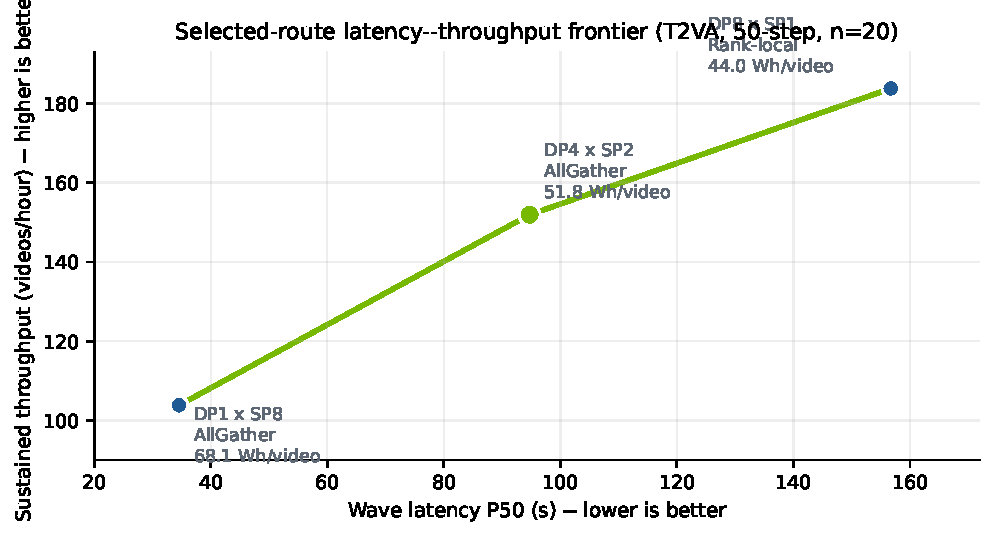
\includegraphics[width=0.82\linewidth]{figures/pareto_frontier.pdf}
\caption{T2VA latency--throughput frontier.  Labels include measured
eight-GPU board energy per output.}
\label{fig:pareto}
\end{figure}

\subsection{RQ2: DLO mode is topology-dependent}

\begin{table}[ht]
\centering
\caption{Effect of enabling AllGather relative to rank-local DLO
($n=5$ paired waves/mode).  Negative latency is favorable.}
\label{tab:dlo}
\small
\begin{tabular}{@{}lrrrl@{}}
\toprule
Topology & Throughput & P50 latency & Peak/GPU (RL$\rightarrow$AG) & Decision \\
\midrule
DP1$\times$SP8 & \best{+129.4\%} & \best{--56.6\%} & 26.26$\rightarrow$23.53 GiB & AllGather \\
DP4$\times$SP2 & +2.2\% & --2.2\% & 23.91$\rightarrow$24.97 GiB & AllGather \\
DP8$\times$SP1 & --4.1\% & +3.8\% & 20.03$\rightarrow$94.03 GiB & Rank-local \\
\bottomrule
\end{tabular}
\end{table}

At DP1, AllGather uses the SP group and is not a no-op.  It simultaneously
reduces latency, energy (28.0\%), and measured peak memory.  At DP4 its gain is
small.  At DP8 it is strictly dominated in this workload and produces a large
asymmetric memory peak (Fig.~\ref{fig:dlo}).  The data therefore reject
topology-independent DLO policies.

\begin{figure}[ht]
\centering
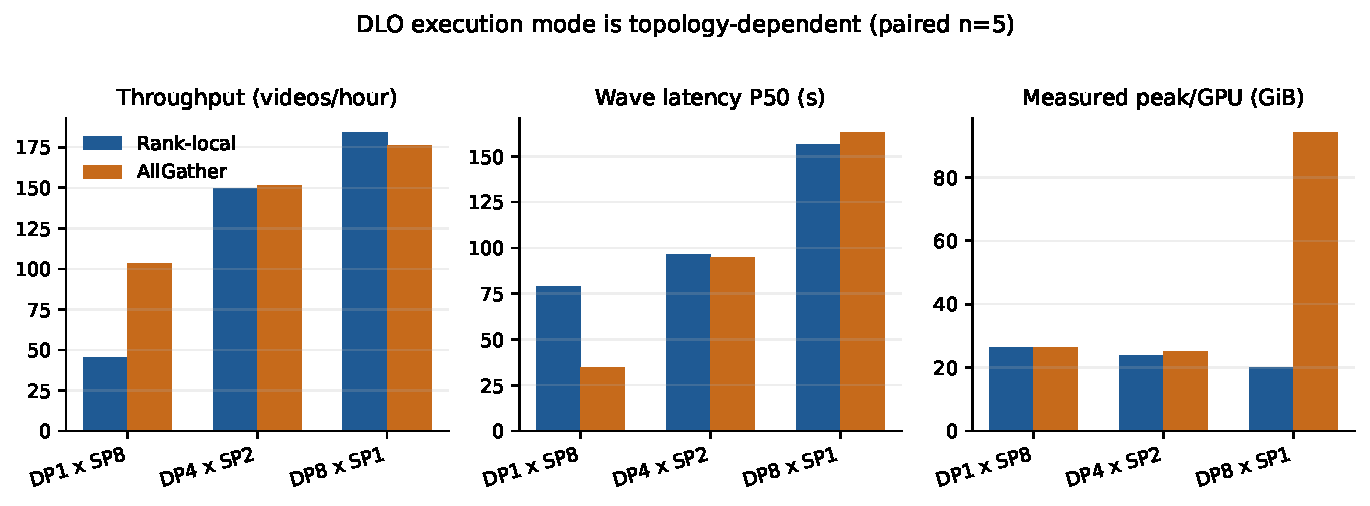
\includegraphics[width=0.96\linewidth]{figures/allgather_ranklocal.pdf}
\caption{Paired DLO-mode comparison.  AllGather's benefit reverses at DP8.}
\label{fig:dlo}
\end{figure}

\subsection{RQ3: Transfer to conditioned generation}

\begin{table}[ht]
\centering
\caption{Best route by service objective for each workload ($n=5$/route).}
\label{tab:transfer}
\small
\begin{tabular}{@{}lrrr@{}}
\toprule
Workload & Lowest P50 latency & Highest throughput & Lowest energy \\
\midrule
FL2VA first-frame & DP1/AG: 37.92 s & DP8/RL: 165.93 videos/h & DP8/RL: 46.88 Wh \\
Ref2VA image+audio & DP1/AG: 55.44 s & DP8/RL: 100.07 videos/h & DP8/RL: 74.06 Wh \\
\bottomrule
\end{tabular}
\end{table}

Conditioning changes scale but not direction: DP1/AllGather remains the
latency route and DP8/rank-local remains the throughput/energy route
(Fig.~\ref{fig:transfer}).  Memory does not transfer as cleanly.  Ref2VA
AllGather approaches 100 GiB/GPU, while DP8/rank-local measures 19.36 GiB.

\begin{figure}[ht]
\centering
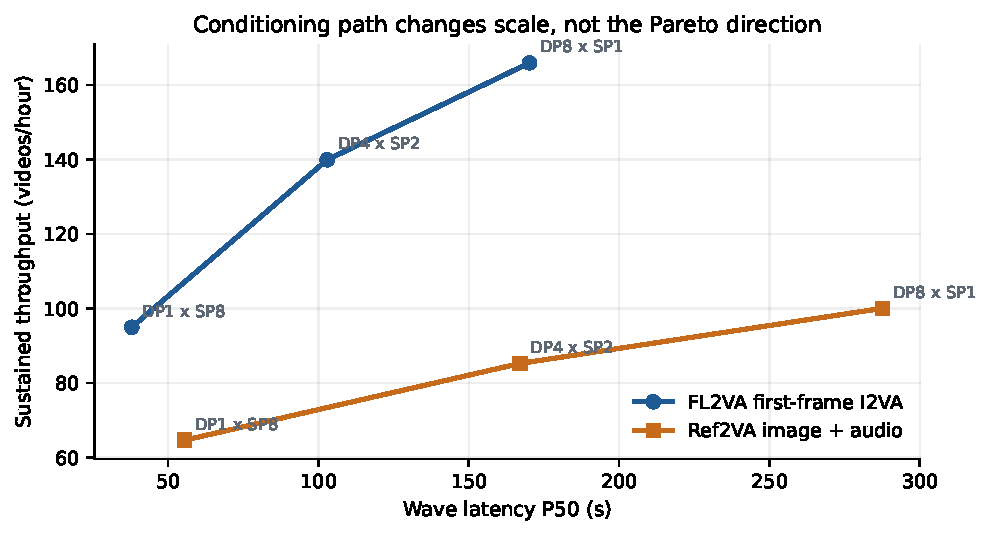
\includegraphics[width=0.77\linewidth]{figures/multimodal_frontiers.pdf}
\caption{FL2VA and Ref2VA frontiers preserve the T2VA ordering.}
\label{fig:transfer}
\end{figure}

\section{Discussion}

The systems interpretation is simple.  SP converts eight GPUs into latency
reduction for one request; DP converts them into concurrent service capacity.
AllGather is useful when coordinated weight movement offsets transfer
overhead, but becomes harmful when collective state and memory concentration
dominate.  Because this crossover occurs within one node and model, DLO mode
should be selected as part of the topology, not as a model-wide switch.

The production policy supported by these measurements is:
\textbf{DP1$\times$SP8/AllGather} for latency-sensitive traffic,
\textbf{DP4$\times$SP2/AllGather} as the balanced default, and
\textbf{DP8$\times$SP1/rank-local} for sustained high queue depth.

\section{Evaluation Integrity and Limitations}

The first DP4$\times$SP2 Ref2VA warmup exposed a correctness defect:
subgroup collectives used global \texttt{src=0} when the group did not contain
global rank zero.  Eight broadcast sites were repaired locally using
\texttt{dist.get\_global\_rank(group, 0)}.  A two-step image+audio smoke
passed before the complete five-wave rerun; failure, smoke, and rerun artifacts
were kept separate.  This fix is not claimed to be part of PR~\#5911.

All successful cases passed output-shape checks without OOM, worker death,
segfault, attention operation-creation failure, or post-fix group-rank error.
Seven cases exhibited a non-fatal 30 s orchestrator-stop delay after output;
the final external check found all GPUs at zero memory and utilization.

The study is limited to one B300 node, one input set, BF16, one resolution and
frame count, and batch size one per replica.  Board energy excludes host and
facility power.  Shape checks do not establish perceptual quality.  Twenty
T2VA waves across two lifecycles characterize steady state but do not
constitute a long-duration SLA or failure-injection campaign.  The local fix
and version mismatch should be resolved before production qualification.

\section{Artifact Availability}

The HTML edition, this PDF, 15-case CSV, 105 wave samples, environment/input
hashes, local source diff, and benchmark runners are archived at
\url{https://github.com/lishunyang12/vllm-omni-rankings/tree/main/scripts/minimax_h3_b300_dlo_industrial_report}.

\begin{thebibliography}{9}
\bibitem{vllmomni}
P. Yin et al., \emph{vLLM-Omni: Fully Disaggregated Serving for Any-to-Any
Multimodal Models}, arXiv:2602.02204, 2026.
\url{https://github.com/vllm-project/vllm-omni}.

\bibitem{minimaxh3}
MiniMaxAI, \emph{MiniMax-H3 model card}, 2026.
\url{https://huggingface.co/MiniMaxAI/MiniMax-H3}.

\bibitem{pr5864}
S. Li, \emph{Fix DLO DP concurrent request execution}, vLLM-Omni PR \#5864,
2026. \url{https://github.com/vllm-project/vllm-omni/pull/5864}.

\bibitem{pr5911}
S. Li, \emph{Enable independent requests for rank-local DLO DP}, vLLM-Omni PR
\#5911, 2026. \url{https://github.com/vllm-project/vllm-omni/pull/5911}.
\end{thebibliography}

\end{document}
